\documentclass{article}
\usepackage[utf8]{inputenc}
\usepackage{amsfonts}
\usepackage{algorithm}
\usepackage{algorithmic}
\usepackage{graphicx}
\usepackage{booktabs}

\title{Small Sample Learning GAN Implementation}
\author{}

\begin{document}

\maketitle

\section{Main Experimental Results}

The results are in Table \ref{tb:mini-imagenet}

\begin{table}[!htbp]
\centering
\caption{Mini-ImageNet Result: table items are [test result] ([valid result]) }\label{tb:mini-imagenet}
\begin{tabular}{cccc}
\toprule
Model & 5-way 1-shot & 5-way 5-shot\\
\midrule
Baseline   (Chen et al., 2019) & 42.11         & 62.53        \\
Baseline++ (Chen et al., 2019) & 48.24         & 66.43        \\
\midrule
DVE-Gauss (w/o pretrain trick) & $\approx$ 43  & $\approx$ 63 \\
DAE-Gauss (w/o pretrain trick) & $\approx$ 44  & $\approx$ 64 \\
ProtoNet  (w/0 pretrain trick) & 44.42         & 64.24         \\
ProteNet+ (w/o pretrain trick) & 48.91 (48.12) & 66.52 (65.13) \\
\midrule
ProtoNet                       & 46.61         & 65.77         \\
DVE-Gauss                      & 46.43 (46.60) & 66.92 (66.99) \\
DAE-Gauss                      & 47.37 (48.53) & 66.99 (68.18) \\
DVE-vMF                        & 51.00 (50.92) & 67.90 (66.67) \\
DAE-vMF                        & 52.02 (52.08) & 66.35 (67.89) \\
\bottomrule
\end{tabular}
\end{table}

\section{Comments}

\begin{itemize}
    \item About DAE (Discriminative Adversarial autoEncoder) model: use one amortized disriminator instead of $K$ discriminators, a extension of Adversarial Autoencoder with supervised labels (+ discriminative loss, + trainable embedding) (Fig \ref{ae})
    \item Preprocessing matters in Mini-ImageNet dataset: Chen et al. (2019) A Closer Look at Few-shot Classification
        \begin{itemize}
            \item Data augmentation
            \item Careful design of output layer
        \end{itemize}
    \item Mini-Imagenet is a noisy dataset
        \begin{itemize}
            \item pretrain trick used in DVE (use BN/Dropout/Rotate Data Augmentation to train a CNN embedding)
                \begin{itemize}
                    \item Rotate Data Augmentation: prevent the pretrained CNN overfitting the data (which will make feature sparse)
                    \item Dropout: If don't use dropout, the performance of DVE will be 45/64
                \end{itemize}
            \item validation perf and test perf might not correlated after converge.
        \end{itemize}
    \item For DAE Implementation
        \begin{itemize}
            \item DAE could not be able to end-to-end learn a embedding (data or mini-imagenet itself).
            \item DAE requires a high learning rate for embedding and unstable training process for embedding matching training process.
            \item (w pretrain trick) both DAE and DVE seems to be a fine-tuned model (reach optimal after about 5-10 epoches)
        \end{itemize}
\end{itemize}

\begin{figure}
\centering
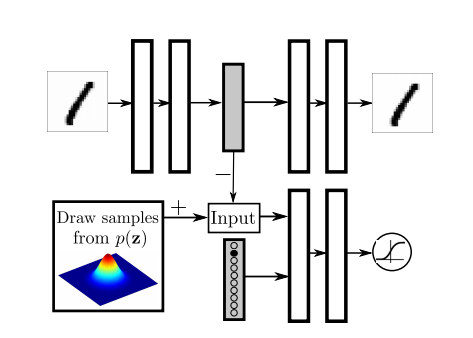
\includegraphics[width=0.8\textwidth]{ae_s.png}
\label{ae}
\caption{Adversarial Autoencoder with supervised labels}
\end{figure}

\end{document}
